 \section{Interactor Role Interaction ODP}\begin{description}
\item [CLASSIFICATION:] Domain Modelling.

\item [MOTIVATION:] Protein Protein Interactions (PPI) are the base for most of the biological processes at a molecular level. For example (http://www.ebi.ac.uk/intact/binary-search/faces/search.xhtml?query=BRCA2).

\item [AIM:] To model different interactions where the interactors can have different roles.

\item [STRUCTURE:] See Figure \ref{odp:Interactor_Role_Interaction_abstract}.
\begin{figure}[]\centering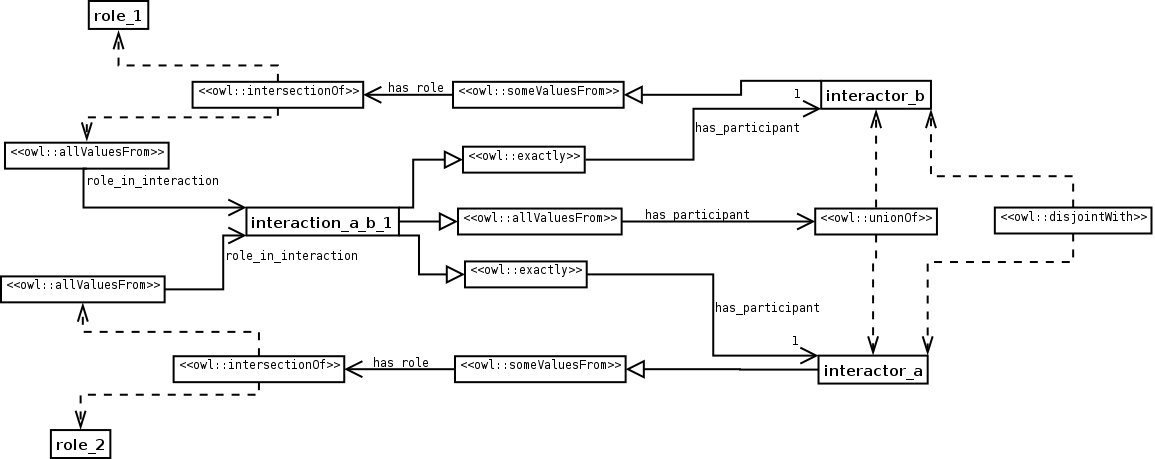
\includegraphics[width=\textwidth]{Catalogue/Interactor_Role_Interaction_abstract}\caption{\label{odp:Interactor_Role_Interaction_abstract} Abstract structure of the Interactor Role Interaction ODP.}\end{figure}

\item [SAMPLE:] See Figure \ref{odp:Interactor_Role_Interaction_instance}.
\begin{figure}[]\centering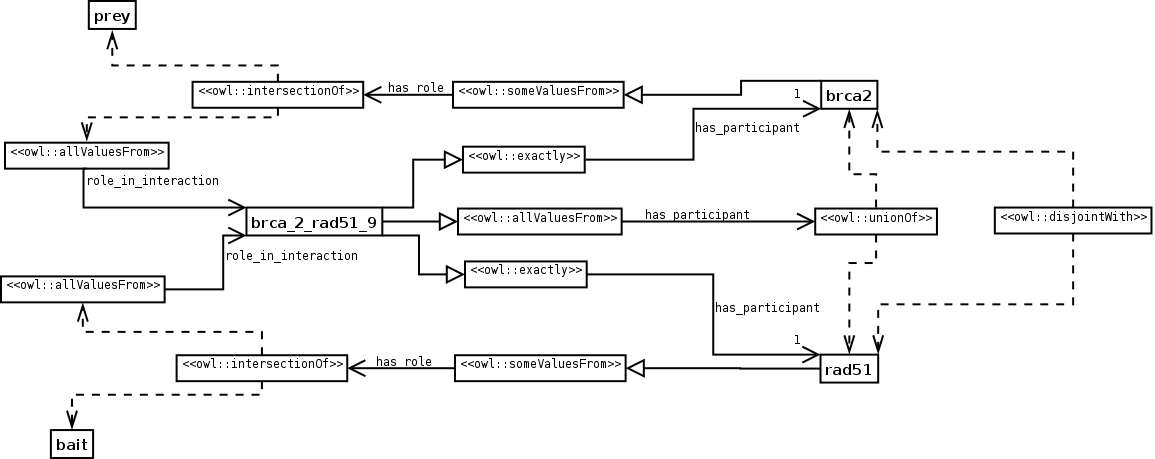
\includegraphics[width=\textwidth]{Catalogue/Interactor_Role_Interaction_instance}\caption{\label{odp:Interactor_Role_Interaction_instance} Sample structure of the Interactor Role Interaction ODP.}\end{figure}

\item [ELEMENTS:] Three object properties are needed: HasRole, RoleInInteraction, and HasParticipant. This ODP has got two aims: close the interactors an interaction can have, and decouple roles from interactions. An interaction is a unique combination of interactors and roles, whereas an interactor can have at the same time many roles and participate in many different interactions (but never with different roles in the same interaction).

\item [IMPLEMENTATION:] The three object properties must be created first (HasRole, RoleInInteraction and HasParticipant). Each interaction bears a closure, so apart of an axiom [HasParticipant exactly 1 InteractorX], an axiom of the type [HasParticipant only (Interactor1 or InteractorN)] should be used. For each interactor, add an axiom of the type [HasRole some (Role and RoleInInteraction Interaction), so queries can be decomposed for roles or participation in interactions, or participations in interactions with certain roles.

\item [RESULT:] The participation events and the role with which interactors participate in concrete interactions are decoupled. Also, each interaction has a given set of interactors and not more.

\item [ADDITIONAL INFORMATION:] See also the following paper: M. Dumontier. Biological situational modeling: Defining Molecular Roles in Pathways and Reactions. 2008. OWL Experiences and Design (OWLED-EU 2008).

\item [REFERENCES: ] ~\begin{itemize}
\item \url{http://odps.sourceforge.net}
\item \url{http://www.cellcycleontology.org/}\end{itemize}
\item [URL: ] \url{http://www.gong.manchester.ac.uk/odp/owl/Domain_Modelling_ODP/Interactor_Role_Interaction.owl} \end{description}